\documentclass[11pt]{article}
\usepackage[pdftex]{graphicx}
\usepackage{siunitx}
\usepackage{amsmath}
\usepackage{fixmath}
\usepackage[czech]{babel}
\usepackage[utf8]{inputenc}
\usepackage[T1]{fontenc}
\usepackage{enumitem}
\graphicspath{ {./images/} }
\sisetup{detect-weight=true, detect-family=true}
\begin{document}

\begin{titlepage}
\center


\textbf{\Huge{Signals and systems}}
\\[4.0cm]

\textsc{\Huge {Project}}
\\[0.2cm]

\Large {Systém pro vyhledávání v audiu pomocí akustického vzoru}
\\[3.0cm]

\Large{Ladislav Ondris (xondri07)}
\\[0.7cm]
\Large{19. 11. 2019}

\end{titlepage}

\newpage

\section{Recordings}
\par

\begin{center}
\begin{tabular}{ |c|c|c| } 
 \hline
 File name & Samples read & Length (seconds) \\ 
 \hline
 sa1.wav &  71658 & 4.478625 \\ 
 sa2.wav & 56298 & 3.518625 \\ 
 si1446.wav & 99818 & 6.238625 \\ 
 si2076.wav & 44778 & 2.798625 \\ 
 si816.wav & 65258 & 4.078625 \\ 
 sx186.wav & 52458 & 3.278625 \\ 
 sx276.wav & 60138 & 3.758625 \\ 
 sx366.wav & 78058 & 4.878625 \\ 
 sx6.wav & 51178 &  3.198625 \\ 
 sx96.wav & 60138 & 3.758625 \\ 
 \hline
\end{tabular}
\end{center}
\par 
The recordings can be used for: 
\par
c) for (a), (b) and for freely available “Czenglish TIMIT” database. 

\section{Queries}
\begin{center}
\begin{tabular}{ |c|c|c|c| } 
 \hline
 File name & Samples read & Length (seconds) & Query \\ 
 \hline
 q1.wav &  12196 & 0.762250 & essentially \\ 
 q2.wav & 12604 & 0.787750 & exercise \\ 
 \hline
\end{tabular}
\end{center}

\section{Spectogram}
\begin{figure}[h]
	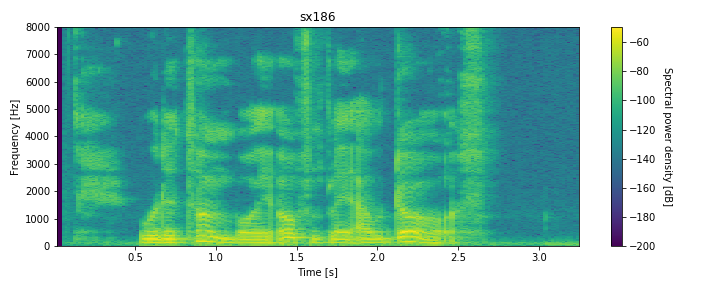
\includegraphics[width=\linewidth]{./sx186_spectogram.png}
	\caption{Would a tomboy often play outdoors?}
\end{figure}

\section{Features}
\par
I used linear bank of filters to calculate features of a given sentence or query. For that I used the matrix multiplication approach $\mathbf{F} = \mathbf{AP}$. 
\par
The purpose of matrix $\mathbf{A}$ is to sum every $B$ rows (in our case 16 rows). To make this work, we create the matrix A by filling it with zeros and ones in a specific pattern so that it produces the sum.
\par 
The first row of the matrix $\mathbf{A}$ will contain 16 ones and the rest of it will be zeros. The second row will contain 16 zeros, then 16 ones, and the rest will be zeros. And so on. 
The shape of the matrix $\mathbf{A}$ is $(B, f.size)$ where $f$ is an array of sample frequencies.

\section{Correlation score calculation}

\section{Main output}
\begin{figure}[h]
	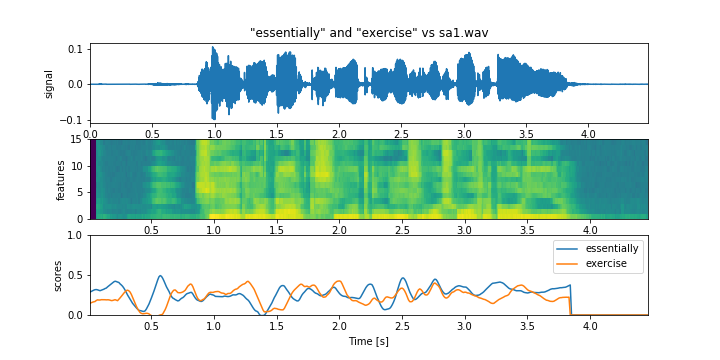
\includegraphics[width=\linewidth]{./docs/sa1.png}
\end{figure}
\begin{figure}[h]
	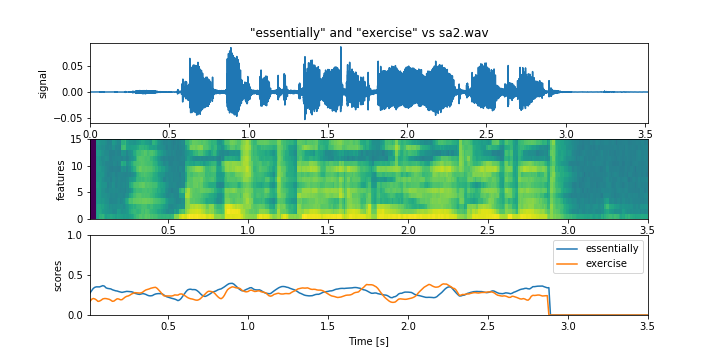
\includegraphics[width=\linewidth]{./docs/sa2.png}
	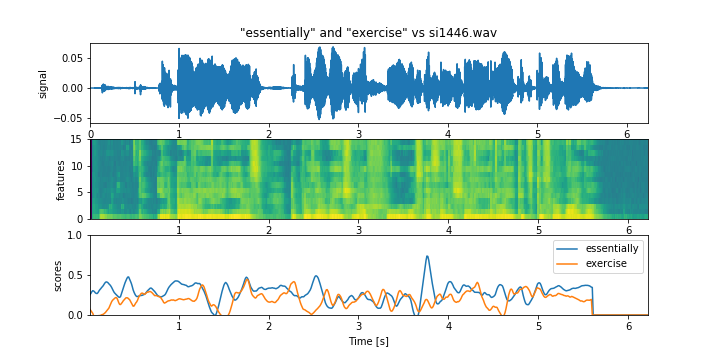
\includegraphics[width=\linewidth]{./docs/si1446.png}
	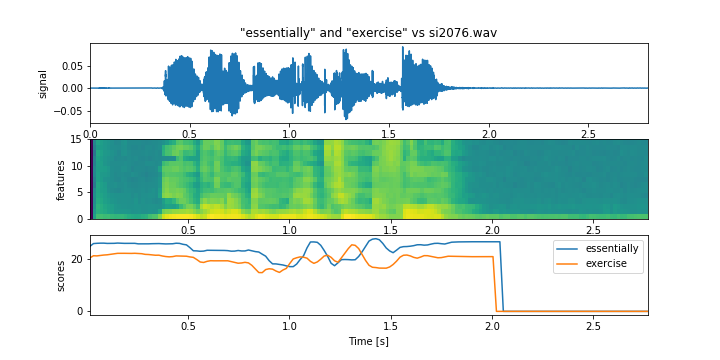
\includegraphics[width=\linewidth]{./docs/si2076.png}
	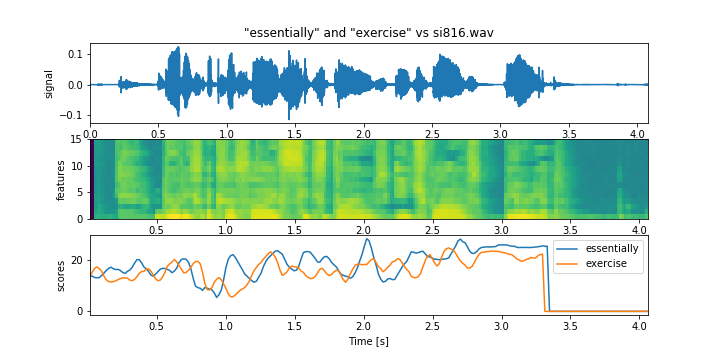
\includegraphics[width=\linewidth]{./docs/si816.png}
	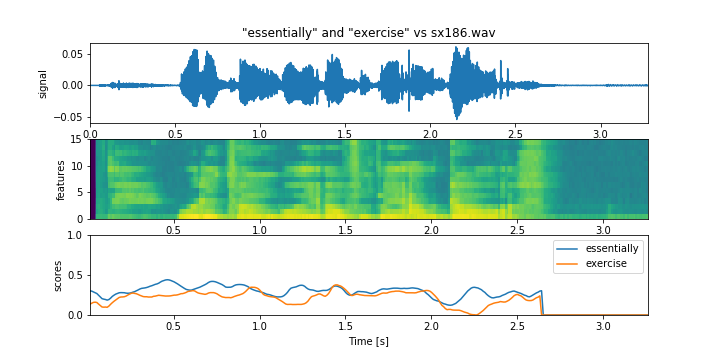
\includegraphics[width=\linewidth]{./docs/sx186.png}
	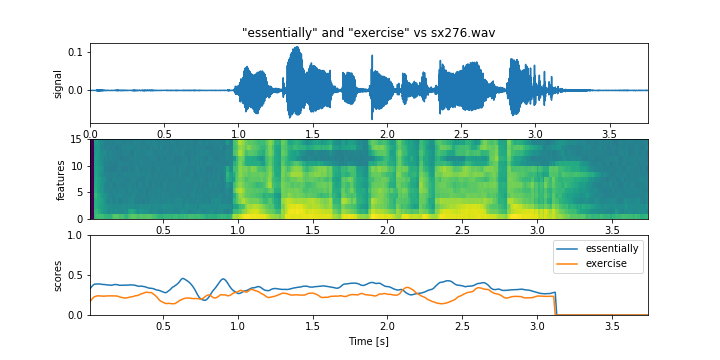
\includegraphics[width=\linewidth]{./docs/sx276.png}
	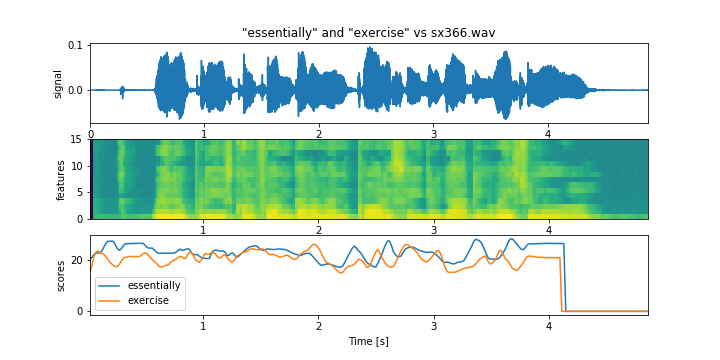
\includegraphics[width=\linewidth]{./docs/sx366.png}
	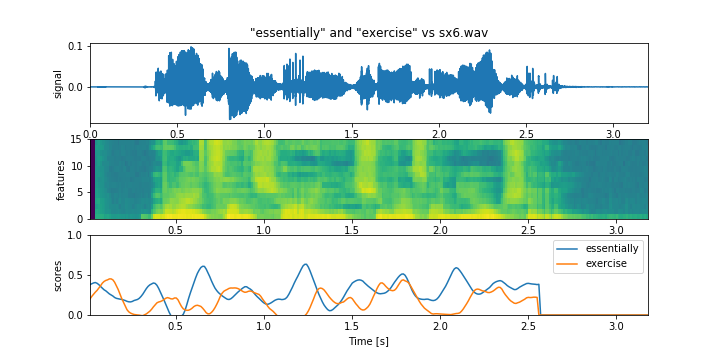
\includegraphics[width=\linewidth]{./docs/sx6.png}
	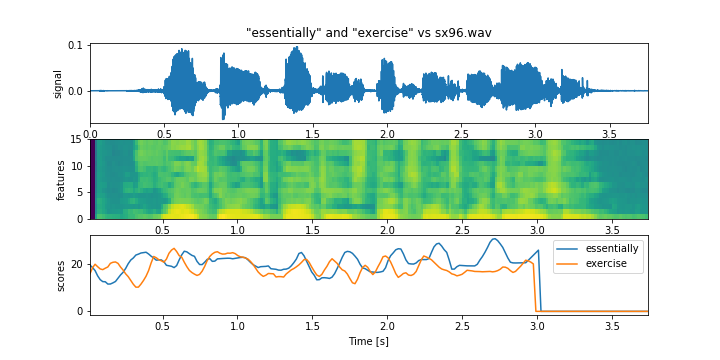
\includegraphics[width=\linewidth]{./docs/sx96.png}
\end{figure}



\end{document}